\documentclass[a4paper,12pt]{article}
\usepackage[utf8]{inputenc}
\usepackage[ngerman]{babel}
\usepackage[top=1in, bottom=1.25in, left=1.25in, right=1.25in]{geometry}
\usepackage{minted}
\usepackage{blindtext}
\usepackage{fancyhdr}
\usepackage{titling}
\usepackage{amssymb}
\usepackage{mathtools}
\usepackage{enumitem}
\usepackage{hyperref}
\usepackage{csquotes}
\usepackage{caption}
\usepackage{subcaption}
\MakeOuterQuote{"}

\hypersetup{colorlinks=true,linkcolor=blue,urlcolor=blue}

\renewcommand{\footrulewidth}{0.4pt}

\setlength\headheight{15pt}
\setlength{\parskip}{1em}

\title{GNS Aufgabe 4}
\author{Eli Kogan-Wang}
\date{\today}

\pagestyle{fancy}
\fancyhf{}
\lhead{\thetitle}
\rhead{\thedate}
\lfoot{\theauthor}
\rfoot{Page \thepage}


\begin{document}
% \maketitle
% \thispagestyle{fancy}
\section{In der Vorlesung haben wir gelernt}

\textbf{dass viele Menschen an einer Farbsehschwäche
  leiden (CVD). Der Chrome Web Store bietet einige Chrome-Erweiterungen an, mit
  denen man die Farbenblindheit auf Websites simulieren kann (Colorblind oder
  Colorblindly). Installieren Sie eine davon und probieren Sie sie auf mehreren Websites
  aus! Führen Sie die folgenden Aufgaben aus:}

Zuerst: Ich verwende den Firefox Browser mit dem eingebauten Feature:
\href{https://firefox-source-docs.mozilla.org/devtools-user/accessibility_inspector/simulation/index.html}{Color vision simulation}
als auch die Software \href{https://www.color-blindness.com/coblis-color-blindness-simulator/}{Coblis}.

\begin{enumerate}[label=\alph*)]
  \item \textbf{Fügen Sie einen Screenshot einer Website bei, die nicht farbenblindenfreundlich
          ist oder Grafiken verwendet, die nicht farbenblindenfreundlich sind, und machen
          Sie Vorschläge zur Verbesserung ihres Designs.}

        Wir verwenden die Website \href{https://html.spec.whatwg.org/multipage/rendering.html}{der HTML Spezifikation}.

        Denn: Die Website verwendet die (in sich selbst beschriebenen) standard-Farben
        für unbesuchte und besuchte Links. Diese sind für Menschen mit einer Protanopie (Rotblindheit),
        Deuteranopie (Grünblindheit) oder Achromatopsie (Farbenblindheit) nicht unterscheidbar.

        % ./2023-05-14-screenshot-without-cvd.png and ./2023-05-14-screenshot-with-cvd.png

        \begin{figure}[h]
          \centering
          \begin{subfigure}[b]{0.4\textwidth}
            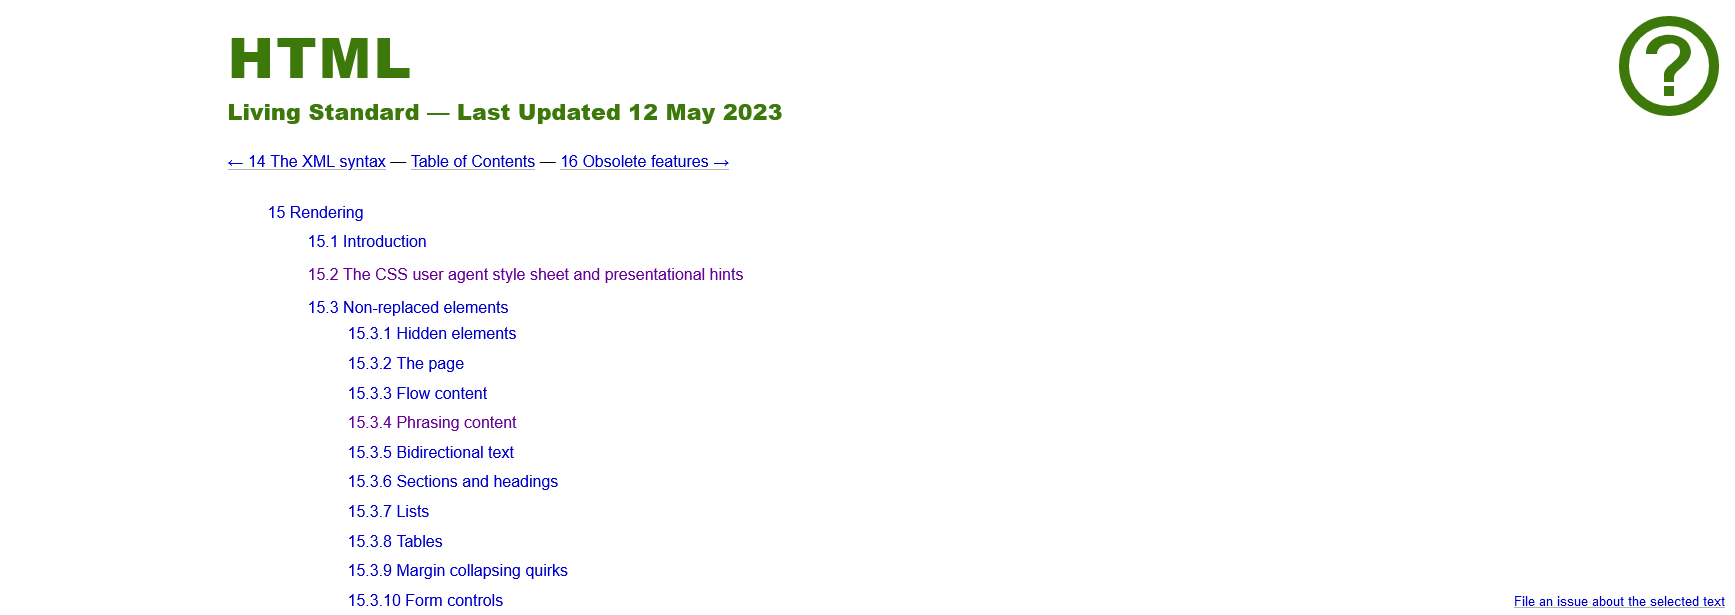
\includegraphics[width=\textwidth]{./2023-05-14-screenshot-without-cvd.png}
            \caption{Ohne Farbsehschwäche}
            \label{fig:without-cvd}
          \end{subfigure}
          \begin{subfigure}[b]{0.4\textwidth}
            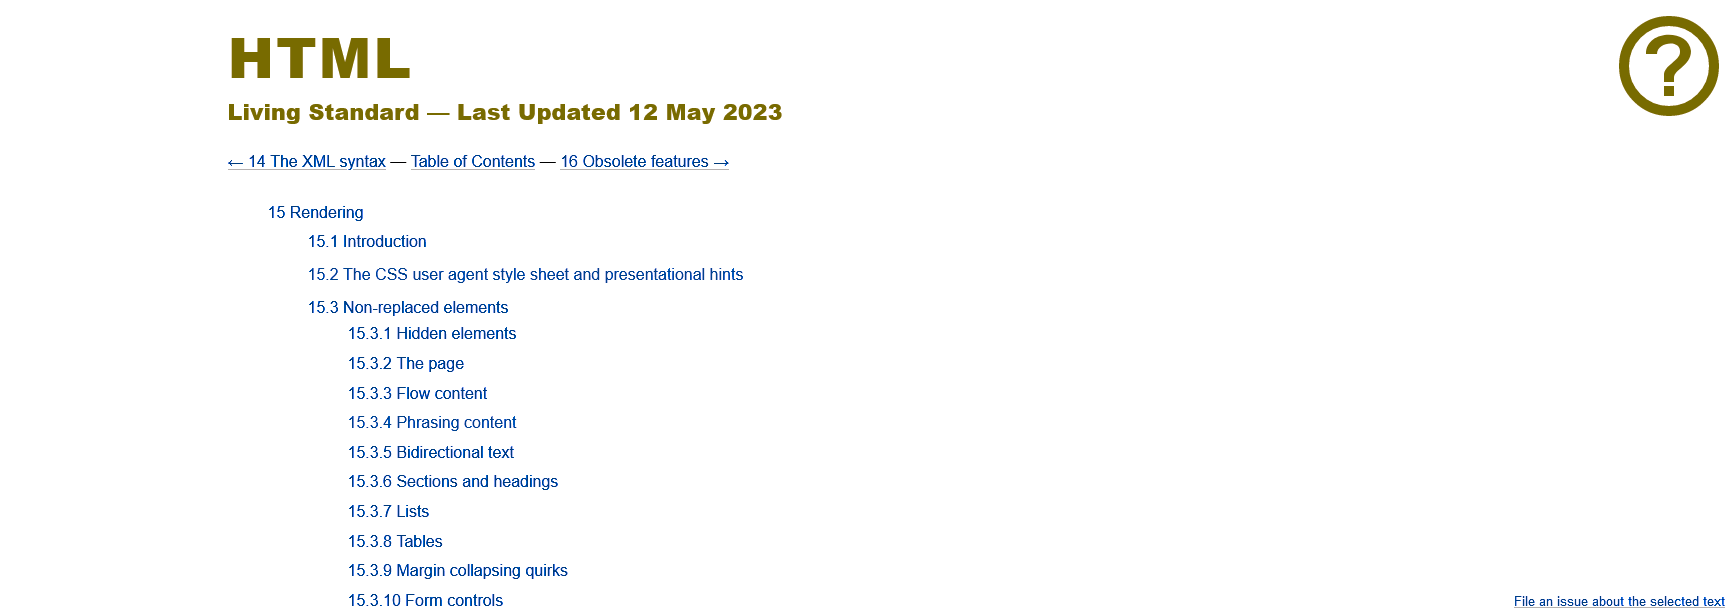
\includegraphics[width=\textwidth]{./2023-05-14-screenshot-with-cvd.png}
            \caption{Mit Protanopie}
            \label{fig:with-cvd}
          \end{subfigure}
        \end{figure}

        Das Problem ist über das gesamte moderne Web verbreitet. Man kann aber als Website-Betreiber
        oder Browser-Nutzer die CSS Farben anpassen, bspw. mit folgendem Snippet:

        \begin{minted}{css}
          a:visited {
            color: gray !important;
          }
        \end{minted}

        Der spezifische Vorschlag für die Farbe "grau" wurde vom Reddit Nutzer
        \href{https://www.reddit.com/r/ColorBlind/comments/n35ht1/bad_website_examples/gwnzs4w/}{/u/macbig273 mit Deuteranomalie} gemacht.
  \item \textbf{Fügen Sie einen Screenshot einer Website bei, die farbenblindenfreundlich ist
          und Grafiken verwendet, die ebenfalls farbenblindenfreundlich sind. Erläutern
          Sie, warum das Design dieser Website besonders gut für Personen mit
          Farbsehschwäche geeignet ist.}

        Wir verwenden die Website \href{https://de.wikipedia.org/wiki/Barrierefreiheit}{Seite „Barrierefreiheit“. In: Wikipedia – Die freie Enzyklopädie}.

        \begin{figure}[h]
          \centering
          \begin{subfigure}[b]{0.4\textwidth}
            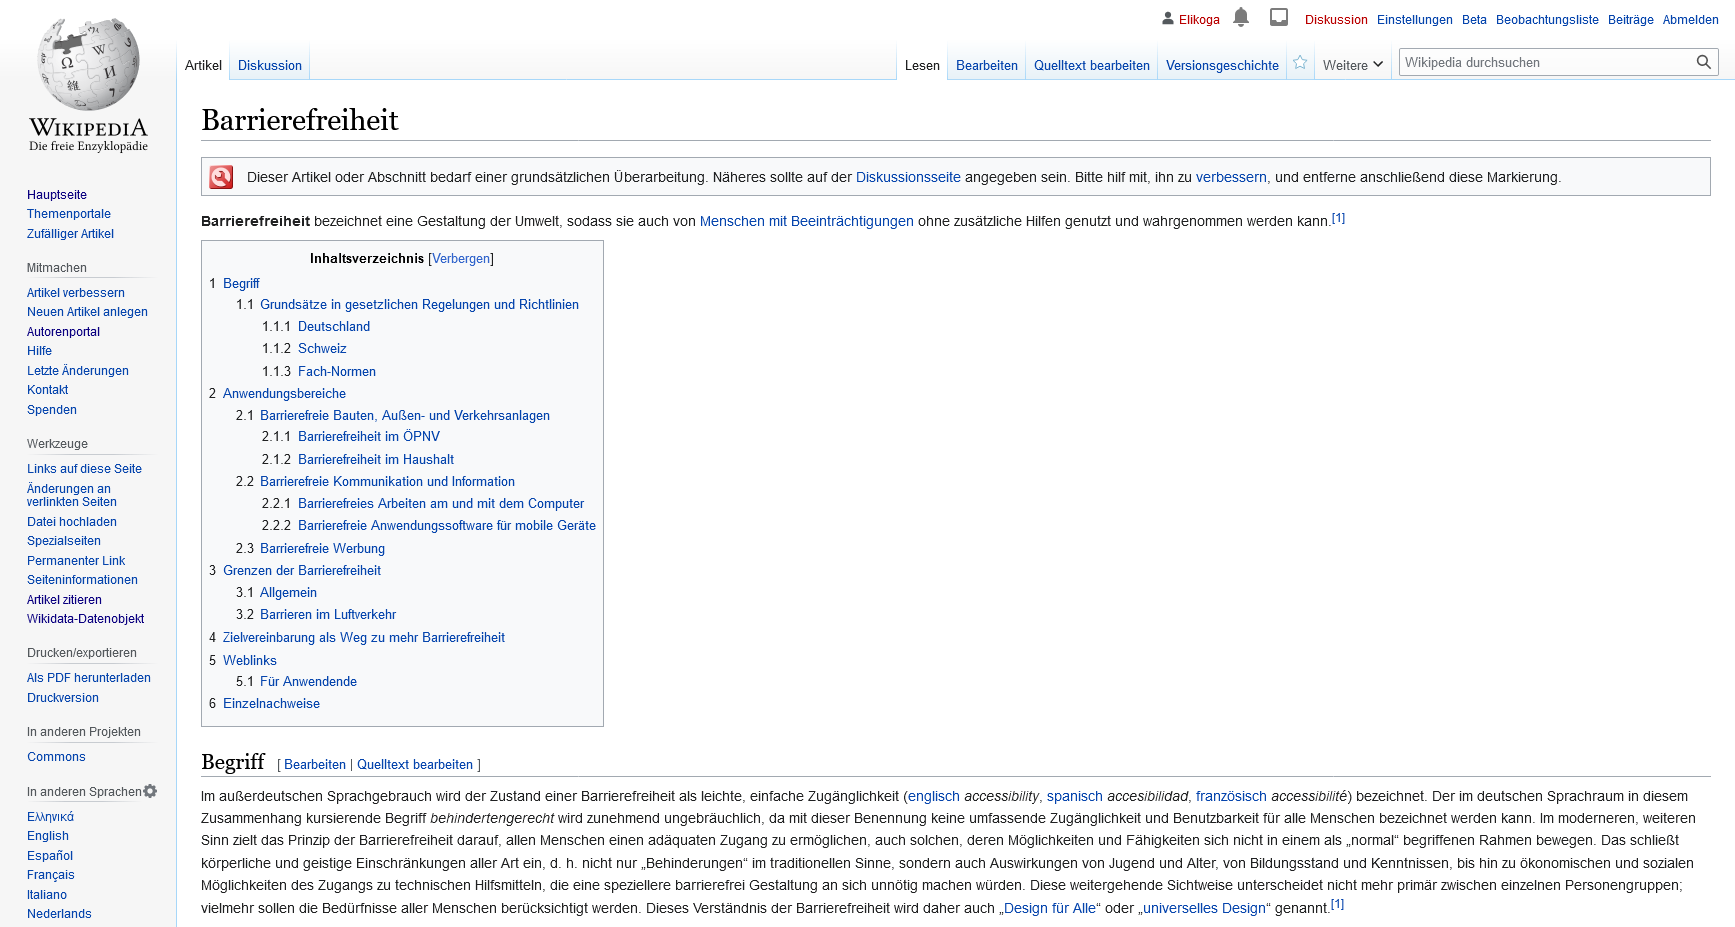
\includegraphics[width=\textwidth]{./2023-05-14-screenshot-without-cvd-wikipedia.png}
            \caption{Ohne Farbsehschwäche}
            \label{fig:without-cvd-wikipedia}
          \end{subfigure}
          \begin{subfigure}[b]{0.4\textwidth}
            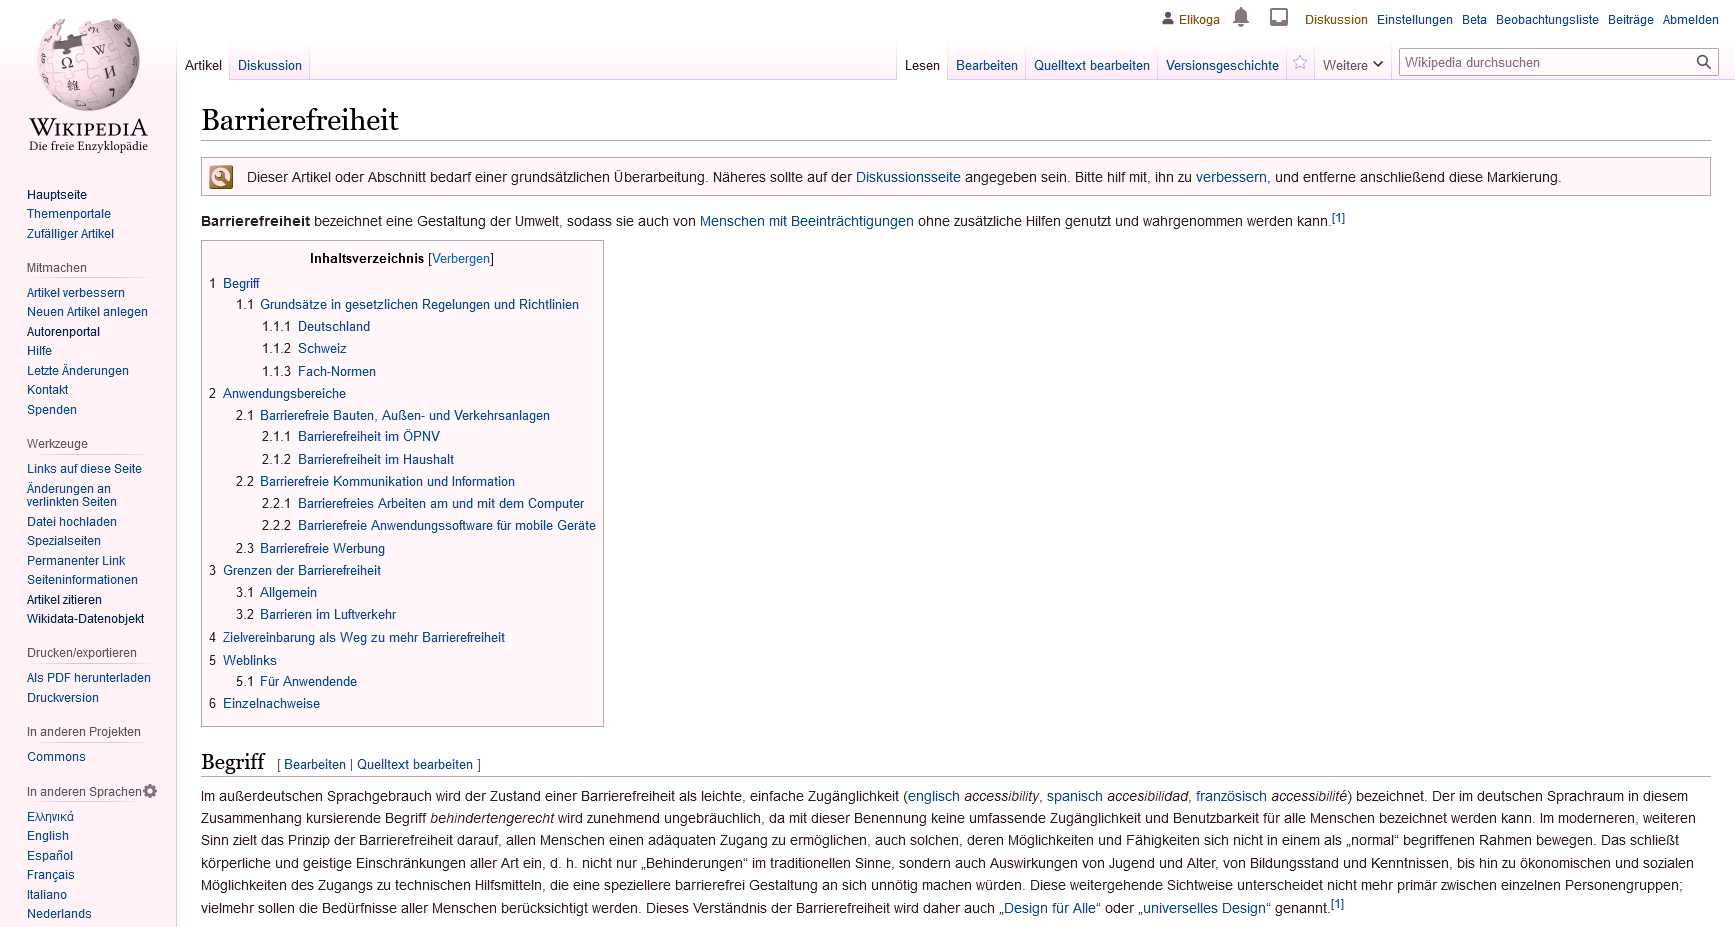
\includegraphics[width=\textwidth]{./2023-05-14-screenshot-with-cvd-wikipedia.png}
            \caption{Mit Deuteranopie}
            \label{fig:with-cvd-wikipedia}
          \end{subfigure}
        \end{figure}

        Wikipedia verwendet die Farben "schwarz" und "weiß" für Text-Vordergrund und Hintergrund.
        In Links verwendet Wikipedia die Farbe "blau" (und "rot" in Außnahmefällen) für Links.

        Die Farbe "blau" ist von Schwarz und Weiß für Menschen mit Protanopie, Deuteranopie oder Tritanopie unterscheidbar.
\end{enumerate}

\section{Unser Designer hat vier UI-Designs für ein Popup vorbereitet}

\textbf{Wählen Sie das Design,
  das Sie für das beste halten, basierend auf den Typografiekriterien, die wir in Vorlesung
  gelernt haben. Erklären Sie, warum Sie sich für dieses Design entschieden haben und
  warum die anderen Designs schlechter sind. Schreiben Sie etwa 1-3 Sätze zu jedem
  Entwurf.}

Wir gehen mit dem Ausschließ-Verfahren vor. Wir schließen Design 3 aus, da der Stil des Haupttextes
eine zu geringe Gewichtung hat. Dadurch wird der Kontrast zwischen Haupttext und Hintergrund
vernachlässigt und der Text wird schwerer lesbar. Zusätzlich ist der hervorgehobene Text (Überschrift, Buttons) zu dick,
sodass im Vergleich der Haupt-Text in den Hintergrund gerückt wird. Im Vergleich mit
den anderen Designs fällt auf, dass die Buttons in gemischter Groß- und Klein-schreibung
beschriftet sind.


Wir schließen Design 1 aus, da es unbedacht den Text in Blocksatz (justified) setzt.
Dadurch werden Abstände zwischen Wörtern vergrößert, was die Lesbarkeit erschwert.
Die Buttons sind mit Großschreibung (uppercase) hervorgehoben.

Wir schließen Design 2 aus, da der Zeilenabstand (leading) zu gering ist. Dadurch wird
die Lesbarkeit erschwert. Zusätzlich fällt auf, dass der Buchstabenabstand (Tracking) klein ist.
Die Buttons sind mit Großschreibung (uppercase) hervorgehoben.

Damit bleibt uns Design 4.
Das Leading und Tracking haben lesbare Werte.
Der Text ist Links-angeordnet, da es ein Text in Paragrafen-Form ist.






\end{document}
